
\title{Lab Report 09 - Shape from Silhouettes}
\author{
        Manuel Galliker  14-921-969 \\
                manuelga@student.ethz.ch
}
\date{\today}

\documentclass[12pt]{article}
\usepackage{graphicx}
\usepackage{float}
\begin{document}
\maketitle


\section{1.  Silhouette extraction  }

In this task a brightness threshhold shall be tuned to give us a good silhouette. The calculation of the silhouette is done in a very simple way by including all the pixels above that threshhold. A good result, covering all of david, was obtained by a threshhold of 112. 

\vspace{5mm}
\begin{figure}[H]
	\centering
	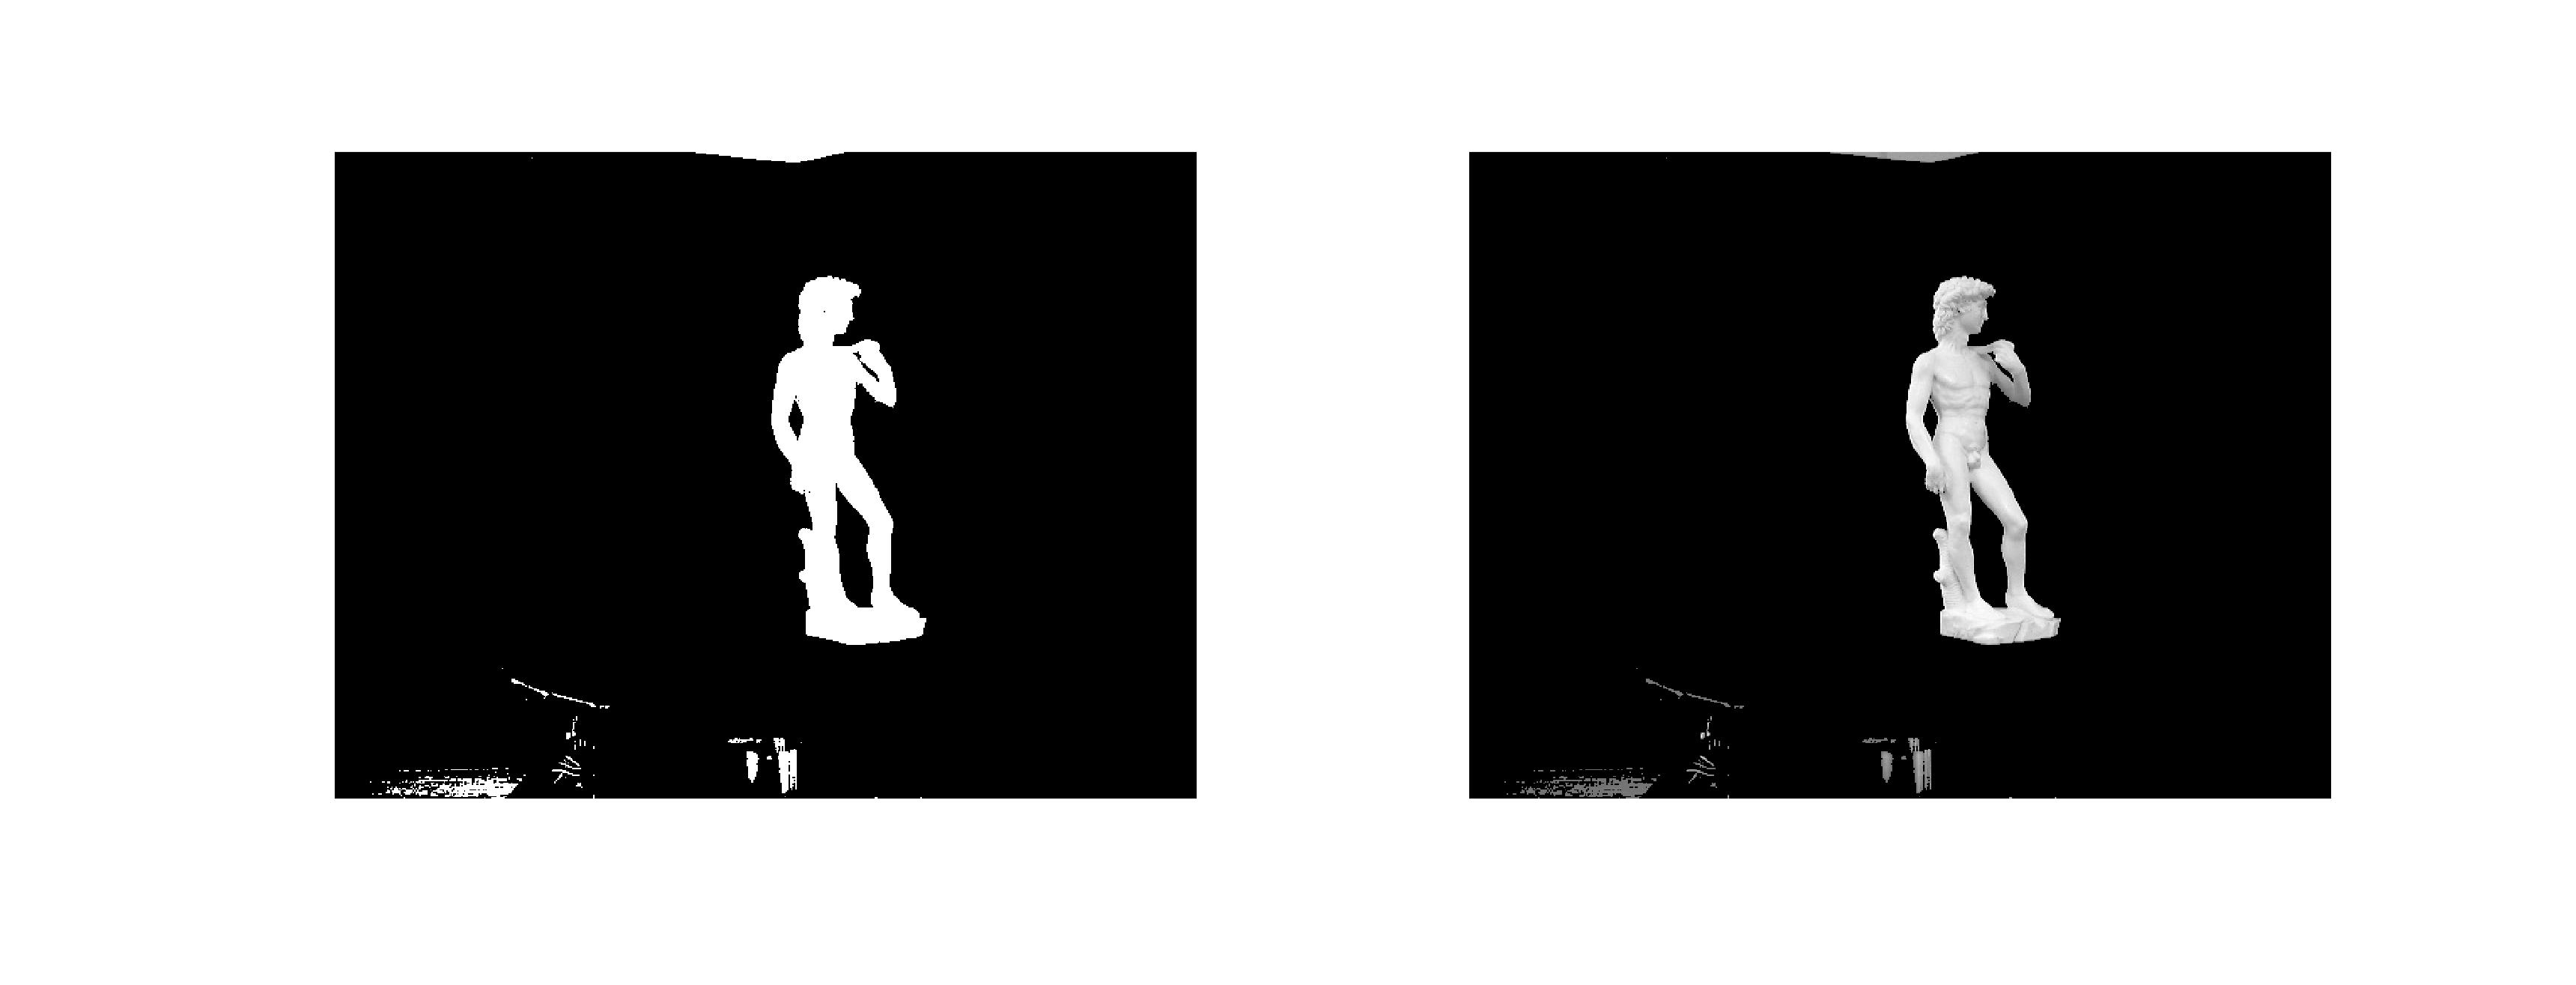
\includegraphics[width=1.1\textwidth]{1.jpg}
	\caption{Silhouette of David for the last image}
	\label{fig1}
\end{figure}
\vspace{5mm}

\section{ Volume of Interest }

The Volume of interest was tuned with the corresponding plot to fit david tightly. The final values are as follows:
$bbox = [0.28 -0.28 -1.9; 2.25 1.3 2.75]$

\vspace{5mm}
\begin{figure}[H]
	\centering
	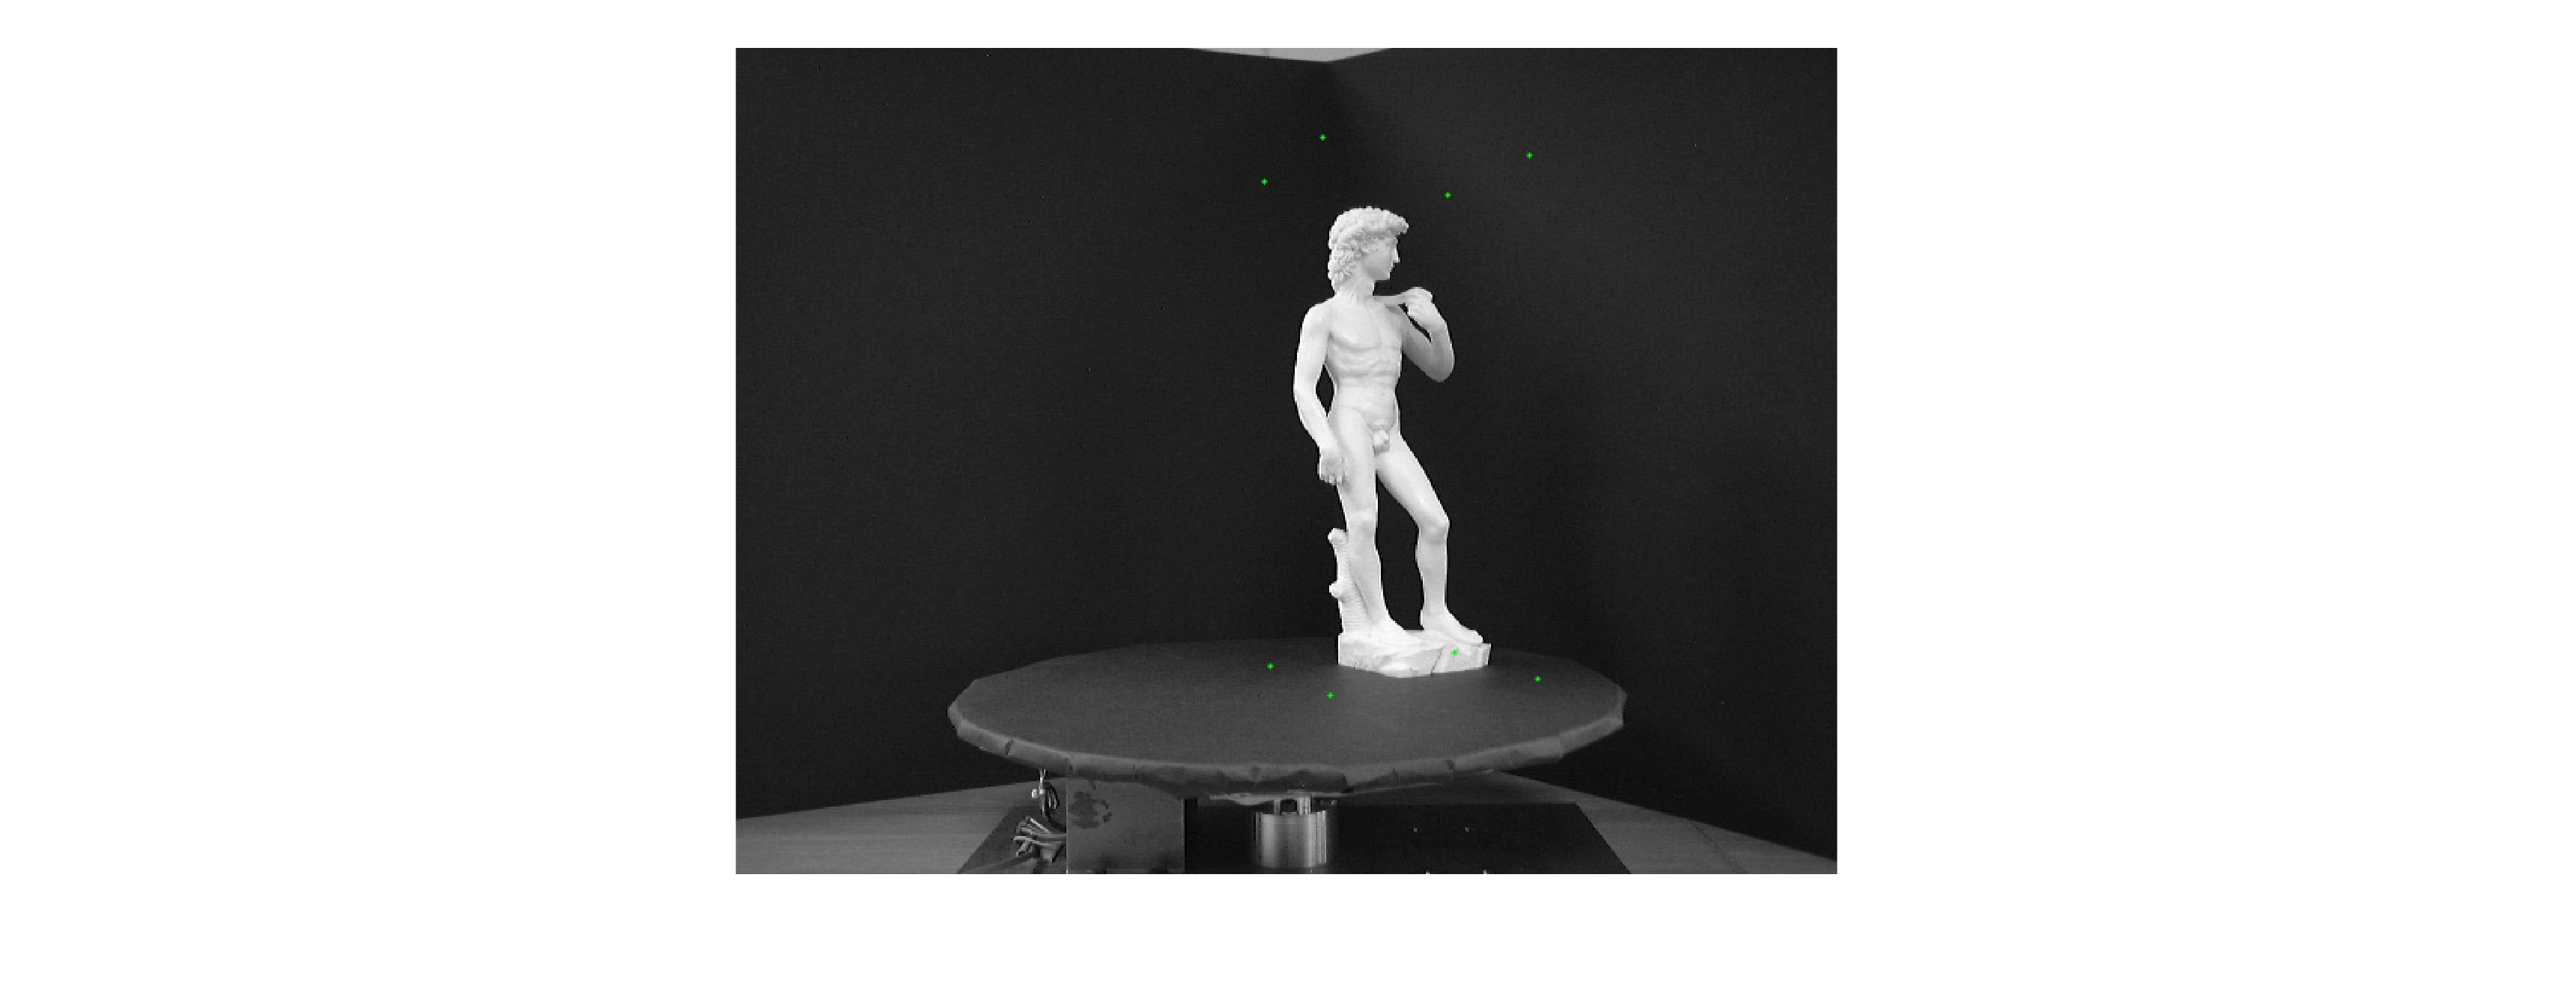
\includegraphics[width=1.1\textwidth]{2.jpg}
	\caption{Box of interest around David for the last image}
	\label{fig1}
\end{figure}
\vspace{5mm}

The resolution of the volume was scaled up to $254x254x512$. At that point a further upscaling would not have given a better result since the resolution of the images themselves were not high enough. The final choice of parameters was:
\vspace{5mm}
\newline
$volumeX = 128$
\vspace{5mm}
\newline
$volumeY = 128$
\vspace{5mm}
\newline
$volumeZ = 256$
\vspace{5mm}
\newline
$volumeThreshold = 17$
\vspace{5mm}
\newline
\section{Visual Hull }

The implementation of the visual hull algorithm was straight forward. In the algorithm for each voxel, defined by the Volume of interest and the resolution, the projection into 2D space is calculated. Then it is checked, whether this point lies within the silhouette. This is then repeated for each picture and the amount of silhouette matches it added. Where the amount of matches is larger than the silhouette threshhold (in this case 17 out of 18 pictures), , the voxel is assumed to be a part of the body. 



\section{Conclusion and Discussion}

As can be seen this approach gives quite a good 3D reconstruction of David. However, this simple approach to calculate the silhouette only works because of the lightning and colouring of the objects being ideal in the provided example. This would not work so well under varying lightning or colour circumstances. 
\newline
An inherit disadvantage of the silhouette approach, is that all the information lying within the silhouette is unused. A human can already with the varying brightness of david due to shadows get an very good idea of a 3D shape. 
\newline
For example a stereo camera setup with a calculated depth map would also give even better result if combined with the Silhouette matching. 

\vspace{5mm}
\begin{figure}[H]
	\centering
	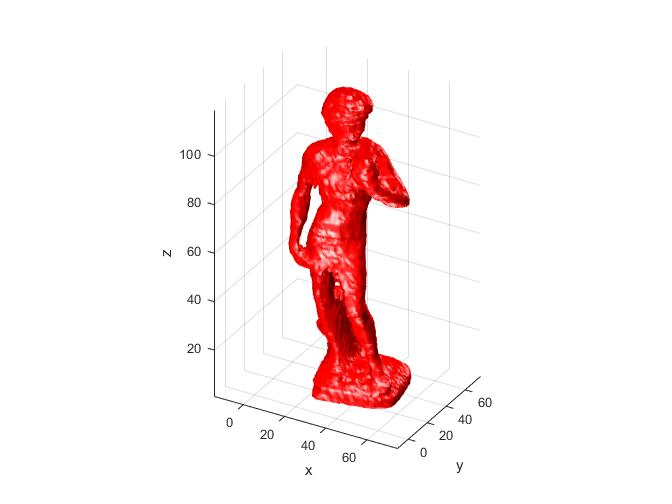
\includegraphics[width=0.9\textwidth]{david_128_1.jpg}
	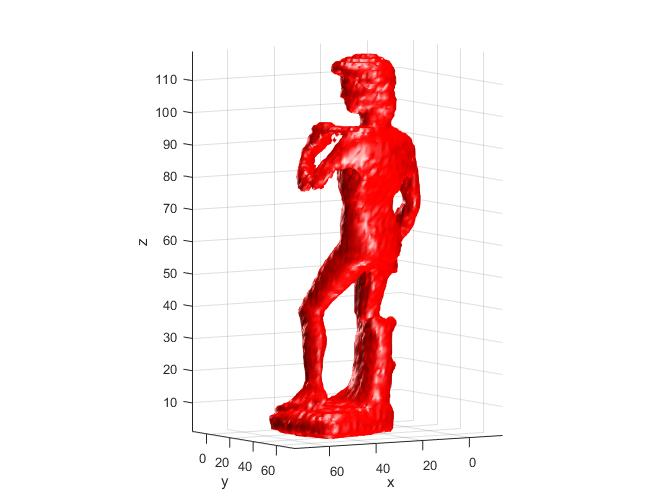
\includegraphics[width=0.9\textwidth]{david_128_2.jpg}
	\caption{3D scan of David using a box resolution of 64x64x128}
	\label{fig1}
\end{figure}
\vspace{5mm}

\vspace{5mm}
\begin{figure}[H]
	\centering
	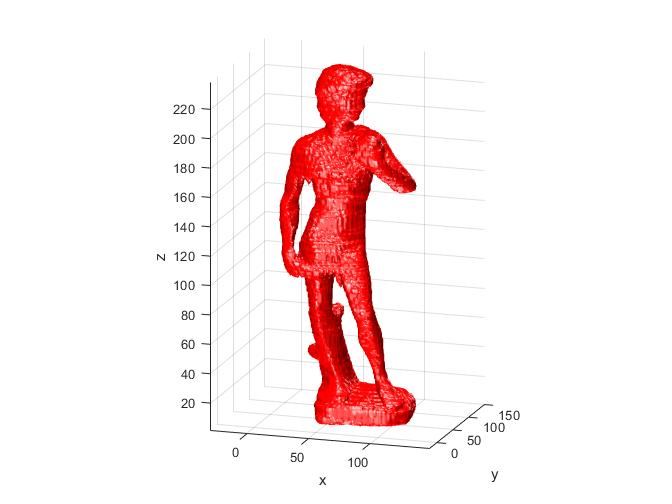
\includegraphics[width=0.9\textwidth]{david_256_1.jpg}
	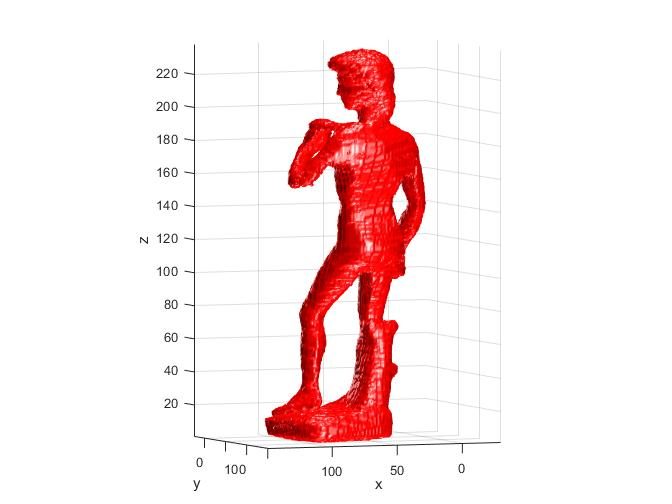
\includegraphics[width=0.9\textwidth]{david_256_2.jpg}
	\caption{3D scan of David using a box resolution of 128x128x256, which was the final choice}
	\label{fig1}
\end{figure}
\vspace{5mm}

\vspace{5mm}
\begin{figure}[H]
	\centering
	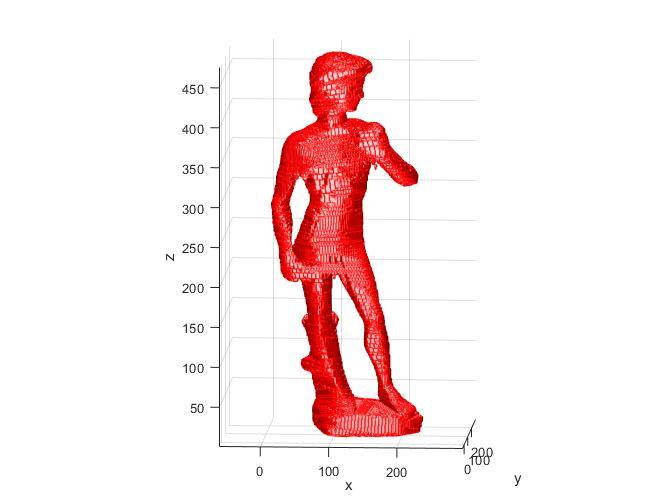
\includegraphics[width=0.9\textwidth]{david512_1.jpg}
	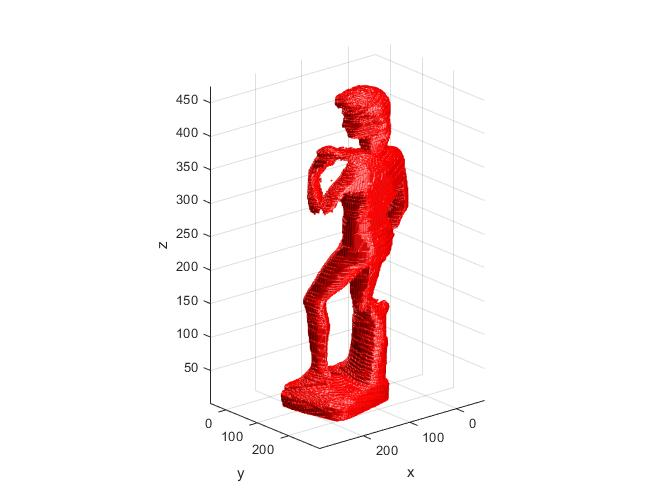
\includegraphics[width=0.9\textwidth]{david512_2.jpg}
	\caption{3D scan of David using a box resolution of 256x256x512}
	\label{fig1}
\end{figure}
\vspace{5mm}


\end{document}